\chapter{红外吸收光谱与拉曼光谱}
\begin{introduction}
    \item 红外光谱及其产生(理解)
    \item 红外光谱仪及其结构(了解)
    \item 红外光谱解谱(熟悉)
    \item 拉曼光谱及其衍生(理解)
\end{introduction}
\section{红外光谱的产生条件及原理}
\begin{definition*}{红外光谱}
    分子能选择性吸收某些波长的红外线,而引起分子中振动能级和转动能级的跃迁,检测红外线被吸收的情况可得到物质的红外吸收光谱,又称分子振动光谱或振转光谱 。
\end{definition*}
\subsection{产生条件}
辐射照射---分子振动---偶极矩变化---产生红外活性

并且辐射也要恰当:
\begin{itemize}
    \item 辐射恰好具有能使物质产生振动跃迁的能量
    \item 辐射与物质间具有耦合作用
\end{itemize}
\begin{note}
    只有发生偶极矩变化($\Delta \mu \neq 0$)的振动才能引起可观测的红外吸收光谱,该分子称为红外活性的。所以对称分子($\Delta \mu=0$)是非红外活性的。
\end{note}
\subsection{振动形式}
\begin{itemize}
    \item 双原子分子振动——“谐振子模型”
    \begin{theorem*}{谐振子模型}
        化学键等于无质量的弹簧连接的两个可视为刚性小球的,质量等于两原子质量的分子模型,其中:
        \begin{equation*}
            \bar{v}=\frac{1}{2\pi c}\sqrt{\frac{k}{\mu}}
        \end{equation*}
        
        其中各符号意义:
            \begin{itemize}
                \item $c$:光速
                \item $k$:键力常数
                \item $\mu$:折合质量$\mu=\frac{m_{1}\cdot m_{2}}{m_{1}+m_{2}}$
            \end{itemize}
    \end{theorem*}
    \item 多原子分子振动
    \begin{itemize}
        \item 伸缩振动——高频区
        \begin{figure}[ht]
            \centering
            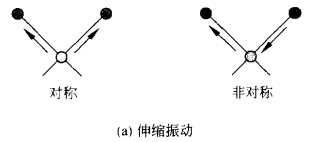
\includegraphics[width=6cm]{image/chp5_flex_vir.png}
            \caption{伸缩振动}
            \label{fig:flex}
       \end{figure}
        \item 弯曲振动——低频区
        \begin{figure}[ht]
            \centering
            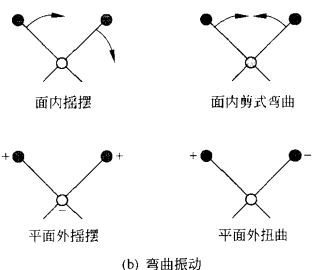
\includegraphics[width=6cm]{image/chp5_twi_vir.png}
            \caption{弯曲振动}
            \label{fig:twist}
       \end{figure}
    \end{itemize}
\end{itemize}

\section{红外吸收仪的结构}
\subsection{色散型红外光谱仪}
\begin{figure}[ht]
    \centering
    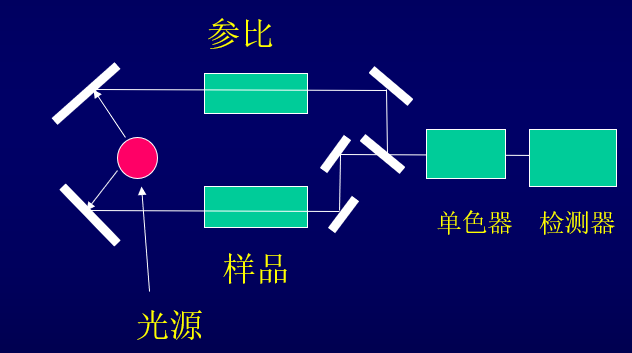
\includegraphics[width=10cm]{image/chp5_ord_ins.png}
    \caption{色散型红外光谱仪}
    \label{fig:ordin_ins}
\end{figure}
\begin{itemize}
    \item 光源:Nerst灯、炭化硅棒等
    \item 单色器
可采用棱镜和光栅
,为了使波长范围增宽,通常可采用几块光栅
。由于红外辐射的强度低,狭缝不能太窄,因此单色性差
    \item 检测器
    \begin{itemize}
        \item 热检测器——热电偶等
        \item 光检测器——\ce{InSb}、\ce{InAs}、\ce{PbSe}等半导体材料,受光照射后导电性变化而产生信号
        \begin{note}
            光检测器的灵敏度比热检测器高几倍,但需要液氮冷却。
        \end{note}
    \end{itemize}
    \item  吸收池
    \begin{itemize}
        \item 固体:\ce{KBr}研磨压片/氧化煤油或重烃调糊
        \item 液体/气体:盐类单晶吸收池(\ce{KBr}/\ce{LiF})
        \begin{note}
强吸收、高分散、不透明的样品,如煤等;常规难制样样
品,如橡胶、高聚物等可采用光声光谱。
        \end{note}
    \end{itemize}

		   
\end{itemize}
\subsection{傅里叶红外光谱仪}
\begin{figure}[ht]
    \centering
    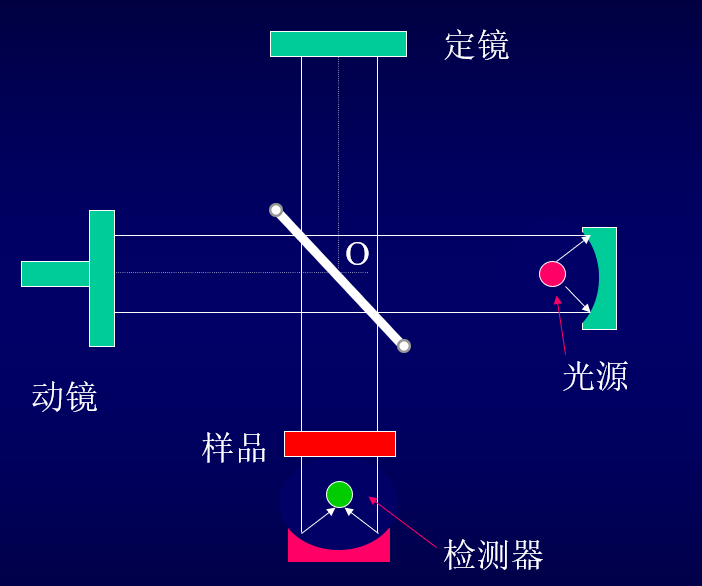
\includegraphics[width=10cm]{image/chp5_fur_ins.png}
    \caption{傅立叶红外光谱仪}
    \label{fig:fur_ins}
\end{figure}
理论基础:
\begin{itemize}
    \item O点与动定镜距离相等——相长干涉
    \item O点到两镜有光程差δ
    \begin{itemize}
        \item $\delta$是$\frac{\pi}{4}$偶数倍——相长干涉
        \item $\delta$是$\frac{\pi}{4}$奇数倍——相消干涉
    \end{itemize}
\end{itemize}

由此,通过傅里叶变换可得该物质红外吸收光谱图
\begin{note}
    傅里叶红外光谱仪的优点:
    \begin{itemize}
        \item 不需要分光,信噪比和灵敏度优良,有利于弱光谱的检测
        \item 扫描速度快
        \item 性能好,价格较低
    \end{itemize}
\end{note}

\section{红外谱图的官能团吸收与谱图解析}
注意:本章图谱分度单位均采用$cm^{-1}$,下文不再重复

\subsection{主要物质的图谱轴}
\begin{itemize}
    \item 4000-2500(X-H)
    \begin{itemize}
        \item O-H	3200-2650
        \begin{itemize}
            \item 气态游离?高频率,波尖
            \item 形成氢键?低频率,波宽
        \end{itemize}
        \item N-H	3650-3200	伯胺有两吸收峰,叔胺无吸收
        \item C-H	3000分界	不饱和>3000 饱和<3000
    \end{itemize}
    \item 2500-2000(三键/累积双键)
    \begin{example}
        C=C, C=N, C=C=C(CO2吸收2365、2335需扣除)
    \end{example}
    \item 2000-1500(双键)
    \begin{itemize}
        \item C=C	1600-1670
        \item 苯环	1450,1500,1580,1600
        \item C=O	脂肪酮:1715左右
        \footnote{取代基会使双键键性减弱,频率下降}
    \end{itemize}
    \item 1500-1300(C-H弯曲振动)
    \begin{itemize}
        \item -$CH_{3}$	1460
        \begin{note}
            1380为谐二甲基特征吸收峰
        \end{note}
        \item -$CH_{2}$-	1470
    \end{itemize}
    \item 1300-910(单键伸缩、分子骨架振动、部分含氢基团弯曲振动)
    \begin{itemize}
        \item C-C	1200
		\item C-O	1100
		\item C-N	1030
    \end{itemize}
    \item 910-
    \begin{itemize}
        \item 苯环取代
        \item 烯的碳氢弯曲振动
    \end{itemize}
\end{itemize}

\begin{note}
    官能团吸收分类:4000-1300 官能团区   1300- 指纹区
\end{note}
\subsection{化合物分类特征吸收}
\subsubsection*{ 烃类化合物特征频率}
\begin{itemize}
    \item 烷烃
    \begin{figure}[ht]
        \centering
        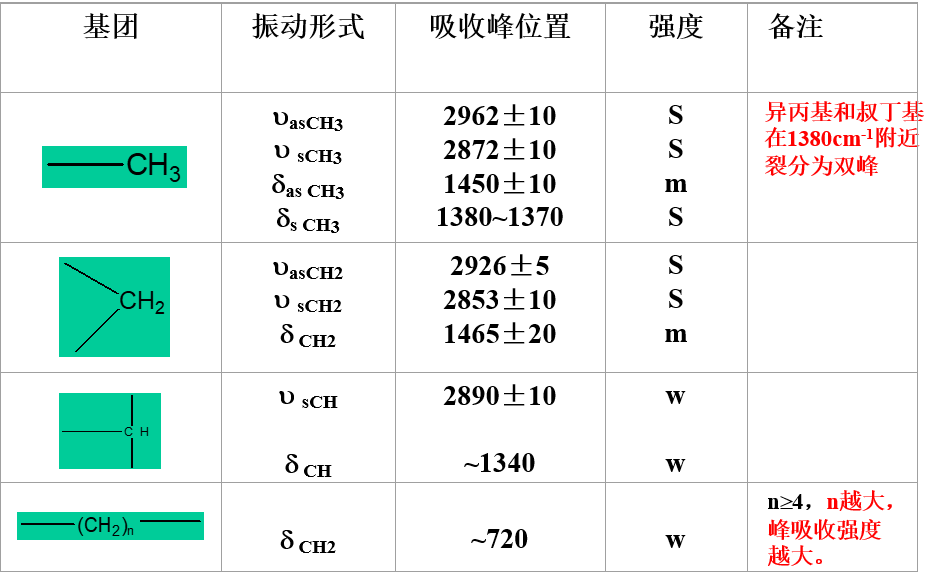
\includegraphics[width=10cm]{image/chp5_ch.png}
        \caption{烷烃特征吸收}
        \label{fig:chp5_ch}
    \end{figure}
    \item 烯烃
    \begin{itemize}
        \item =C-H:3100-3010——1000-800
        \item C=C:1680-1620
    \end{itemize}
    \item 炔烃
    \begin{itemize}
        \item C-H:3310-3300——700-600
        \item C$\equiv$C:2200-2100(当三键位于分子中间时产生)
    \end{itemize}
    \item 芳香烃
    \begin{itemize}
        \item C-H   3000-3100 (芳环C-H伸缩振动)
        \item C=C  1450、1500、1580、1600 (芳环骨架伸缩振动,但后三峰不一定同时出现)
        \item 面外=C-H  900~650  用于确定芳烃取代类型(与芳环取代基性质无关,而与取
        代个数有关,取代基个数越多,即芳环上氢数目越少,振动频率越低。)
        \item 面外=C-H     倍频 2000~1600 cm-1(w)用于确定芳烃取代类型.
        \begin{note}
            如何判断双取代类型? 
            \begin{itemize}
                    \item 邻位:750
                    \item 对位:810-750/725-680/900-860
                    \item 间位:860-800
            \end{itemize}
            \begin{figure}[ht]
                \centering
                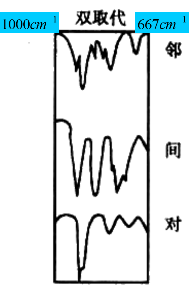
\includegraphics[width=5cm]{image/chp5_double.png}
                \caption{双取代类型判断}
                \label{fig:double}
            \end{figure}
        \end{note}
    \end{itemize}
\end{itemize}
\subsubsection*{醇与酚的特征频率}
\begin{itemize}
    \item 游离OH伸缩振动  3600      尖峰
    \item 缔合OH伸缩振动  3600     又宽又强吸收峰
    \item υC-O             1250-1000   
    \item 面内OH           1500-1300  
    \item 面外OH         650 
\end{itemize}

\subsubsection*{醚的特征频率}
\begin{itemize}
    \item 脂族和环的C-O-C  1150-1070
    \item 脂R-OCH3         2830-2815
    \item 芳Ar-OCH3       ~2850cm-1
\end{itemize}
\subsubsection*{ 胺的特征频率}
\begin{itemize}
    \item -NH2:3390、3290 (双峰)
    \item N-H:1650-1590/900-650(宽)
    \item C-N:
    \begin{itemize}
        \item 1230-1030(脂肪胺)
        \item 1340-1250(芳香胺)
    \end{itemize}
\end{itemize}
\subsubsection*{羰基化合物的特征频率}
\begin{itemize}
    \item C=O:1750-1680(强)
    \item CO-H:2720
\end{itemize}
\begin{figure}[ht]
    \centering
    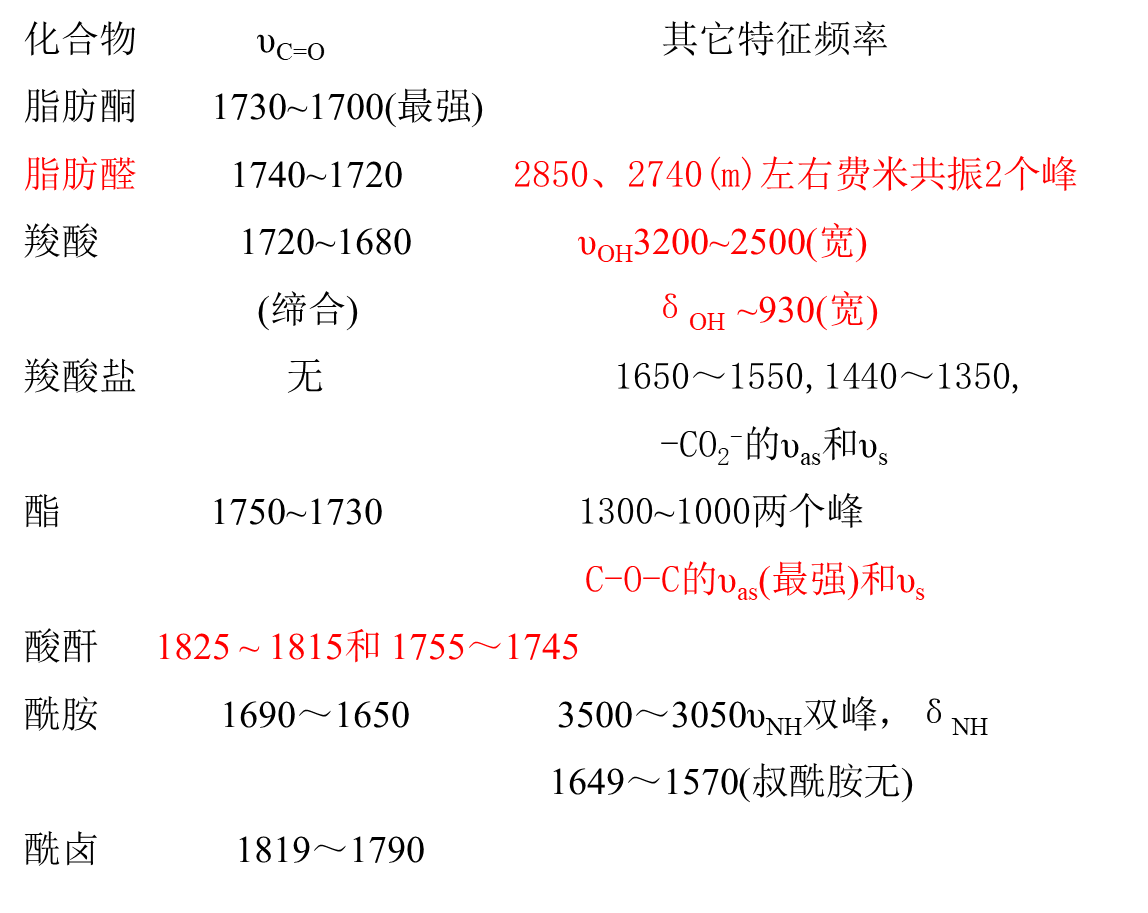
\includegraphics[width=10cm]{image/chp5_co.png}
    \caption{羰基化合物特征吸收}
    \label{fig:chp5_co}
\end{figure}



\subsection{吸收强度与结构的关系}
    i- 基频:由基态跃迁到第一激发态,产生一个强的吸收峰,称为基频峰

    ii- 倍频:由基态跃迁至第二、第三激发态所产生的谱带

    iii- 组合频:两个或两个以上基频之和或之差、或基频与倍频的结合 产生的谱带

    iv- 振动耦合:两个基团相邻且振动频率相差不大时,振动耦合引起吸收频率偏离基频,移向高频或低频方向产生的振动频率

    v- 费米共振:倍频和组合频与某基频相近,相互作用而产生强吸收或发生峰分裂
\begin{note}
    谱图解析一般步骤:三要素:\textcolor{red}{位置、强度、波形}
    \begin{itemize}
        \item (1)根据质谱、元素分析结果得到分子式。
        \item (2)由分子式计算不饱和度U。
        \item (3)观察官能团区,寻找特征官能团
        \item (4)观察指纹区,找苯环取代
    \end{itemize}
\end{note}

\section{拉曼散射与拉曼光谱}
\subsection{拉曼散射与拉曼光谱}
\begin{definition*}{拉曼散射如瑞利散射}
    当光线从一个原子或分子散射出来时,绝大多数的光子,都是弹性散射的,这称为瑞利散射。在瑞利散射下,散射出来的光子,跟射入时的光子,它的能量、频率与波长是相同的。然而,有一小部分散射的光子,散射后的频率会产生变化,通常是低于射入时的光子频率,原因是入射光子和介质分子之间发生能量交换。这即是拉曼散射。
\end{definition*}
\begin{note}
    瑞利散射:弹性碰撞,方向改变而未发生能量交换

    拉曼散射:非弹性碰撞,方向改变并发生能量交换
\end{note}
\begin{figure}[ht]
    \centering
    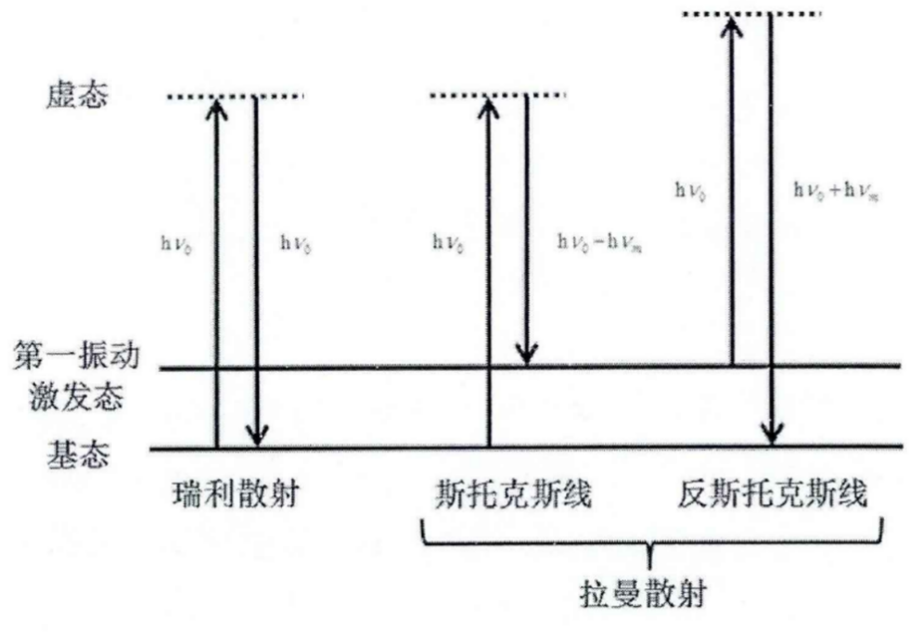
\includegraphics[width=10cm]{image/chp5_sers.png}
    \caption{拉曼散射的产生}
    \label{fig:chp5_laman}
\end{figure}
斯托克斯线:材料吸收能量,导致散射光子能量低于入射光子;

反斯托克斯线:材料失去能量,导致散射光子能量高于入射光子。
\begin{definition*}{拉曼位移}
    斯托克斯线与反斯托克斯线对应频率与入射光频率的差叫做拉曼位移。
\end{definition*}

拉曼散射实质:在交变电场作用下,当分子的振动引起分子极化度$\mu$改变时,则产生拉曼散射

\begin{note}
    拉曼光谱与红外光谱比较:

    拉曼光谱与红外光谱都来自于分子振动,但是
    \begin{itemize}
        \item 具有对称中心的分子,其红外	和拉曼活性是互相排斥的,红外吸收强则拉曼吸收弱。
        
        \begin{example}
            极性基团振动时常伴随偶极矩变化,因而产生较强的红外吸收,非极性基团振动时极化度变化越大,拉曼散射越强,故非极性基团分析常用拉曼光谱
        \end{example}
        \item 凡是没有对称中心的分子,红外和拉曼都是活性的
        \item 对于少数分子的振动,其红外和拉曼光谱都是非活性的。
        \begin{example}
            如乙烯分子的扭曲振动,既没有偶极矩的变化,亦没有极化度的变化,在红外和拉曼光谱中均得不到谱峰。
        \end{example}
    \end{itemize}
\end{note}
\subsection{表面增强拉曼效应}
\begin{definition*}{表面增强拉曼效应}
    表面增强拉曼光谱或表面增强拉曼散射(SERS),是一种通过吸附在粗糙金属表面上的分子或等离子体磁性二氧化硅纳米管等纳米结构增强拉曼散射的表面敏感技术
\end{definition*}

SERS原理:
有两种机理基本不同的理论,实验中仍无法准确地区分它们。
\begin{itemize}
    \item 电磁理论:局部表面等离子体的激发导致SERS的生成
    \item 化学理论:电荷转移配合物的形成导致SERS的生成
\end{itemize},
\begin{note}
    化学理论仅适用于表面已形成化学键的物质,所以不能解释所有观察到的增强信号,而电磁理论可以应用于试样只是物理吸附在表面的情况下。
\end{note}

SERS基质: 
\begin{itemize}
    \item     金属    $\ce{Ag},\ce{ Au}, \ce{Cu},\ce{Ni},\ce{ Al},\ce{ Li},\ce{ Na,} \ce{K}, \ce{Pt}
    $
    \item     半导体  $\ce{CdS}, \ce{Fe_{2}O_{3}}, \ce{TiO_{2}}$
\end{itemize}


SERS活性物质(必须能吸附在基质表面)
\begin{itemize}
    \item 	吡啶等杂环化合物
    \item   苯甲酸衍生物
    \item   氰基衍生物
    \item   一些染料,金属络合物,生物分子,无机分子
\end{itemize}
